\documentclass[compress]{beamer}
\usepackage{ifthen}

\title{Survey Alignment $\to$ Conditions Database}
\author{Dmitry Yakorev, Jim Pivarski, Alexei Safonov}
\institute{Texas A\&M University}
\date{31 May, 2007}

\setbeamertemplate{navigation symbols}{}
\setbeamertemplate{headline}{\includegraphics[height=1 cm]{../cmslogo} \hspace{0.1 cm} \includegraphics[height=1 cm]{../tamulogo} \hfill
\begin{minipage}{9 cm}
\vspace{-0.75 cm} \small
\begin{center}
\ifthenelse{\equal{\insertpagenumber}{1}}{}{\insertsection}
\end{center}
\end{minipage} \hfill
\begin{minipage}{1 cm}
\vspace{-0.75 cm} \small
\begin{center}
\ifthenelse{\equal{\insertpagenumber}{1}}{}{\insertpagenumber/\pageref{numpages}}
\end{center}
\end{minipage}}

%% \xdefinecolor{verylightgray}{rgb}{0.95,0.95,0.95}
%% \beamertemplateshadingbackground{verylightgray}{white}

\begin{document}
\frame{\titlepage}
\section*{Survey $\to$ Database --- Dmitry Yakorev}

\begin{frame}
\frametitle{CSCs have two alignment pins, equidistant from center}

\vspace{-0.75 cm}
\begin{center}
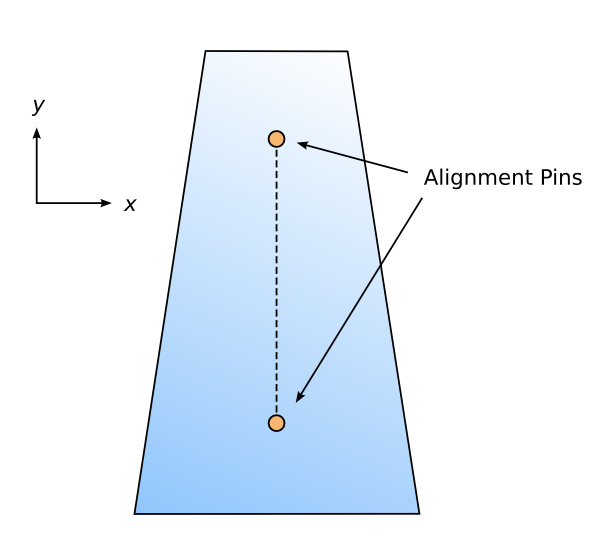
\includegraphics[width=0.65\linewidth]{pins.png}
\end{center}

\vspace{-0.5 cm}
Real positions of these pins measured by photogrammetry
\end{frame}

\begin{frame}
\frametitle{Goal: translate, rotate chamber to match measured}
\only<1>{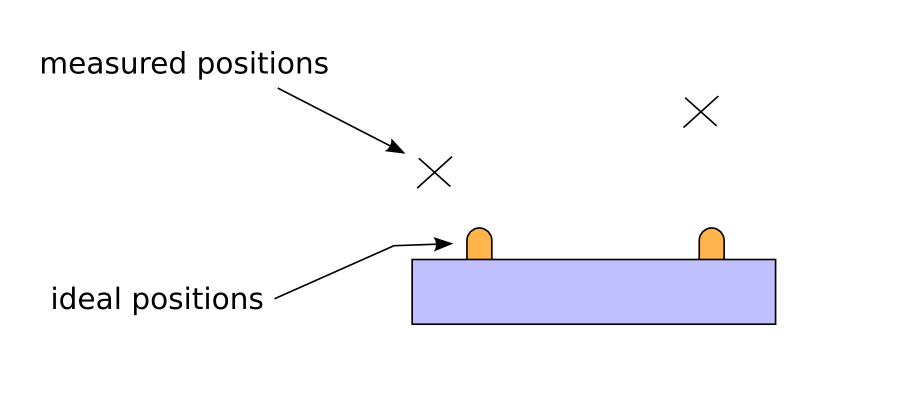
\includegraphics[width=\linewidth]{align1.png}}
\only<2>{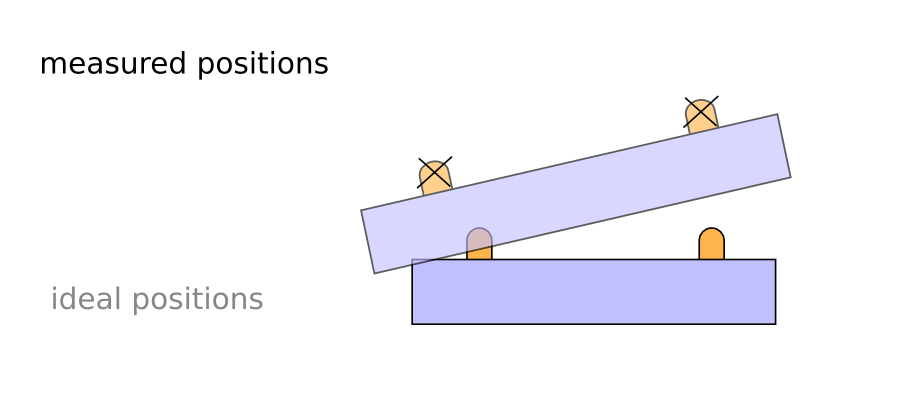
\includegraphics[width=\linewidth]{align2.png}}
\only<3>{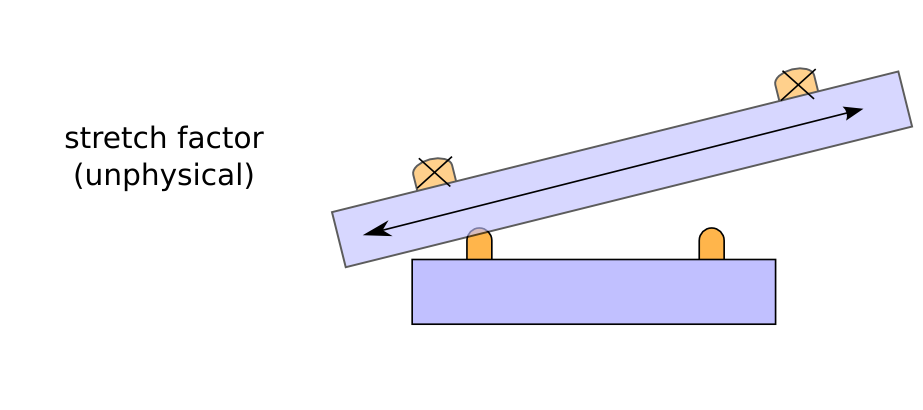
\includegraphics[width=\linewidth]{align3.png}}

\only<1-2>{\vfill Analytic solution: we apply only one motion to the Alignable

\vfill Rotation around $y$ is unconstrained, so we don't touch $\phi_y$}

\only<3>{\vfill Measurement error can stretch a chamber.  Stretch
  is included in formal solution but not applied to Alignable.}
\end{frame}

\begin{frame}
\frametitle{Calculation in detail}
\only<1>{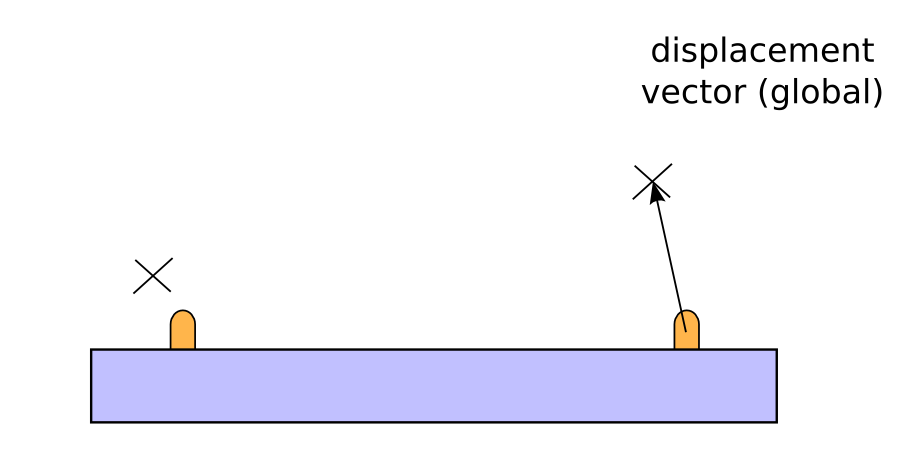
\includegraphics[width=\linewidth]{test.png}}
\only<2>{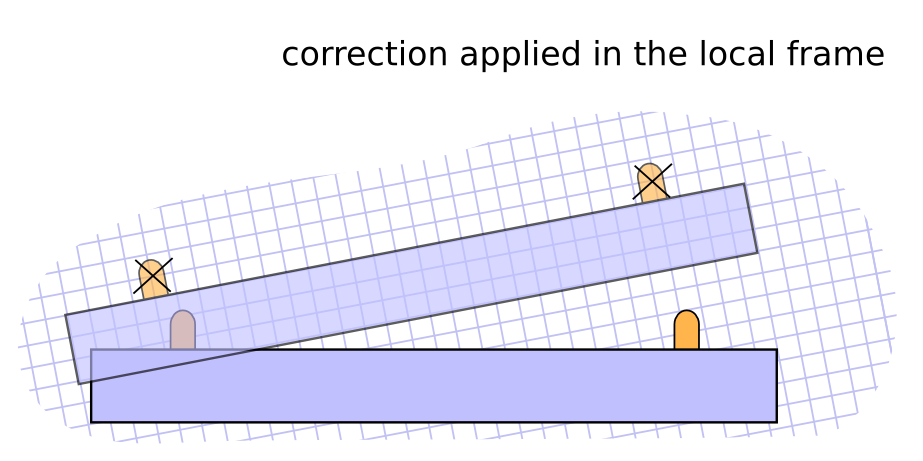
\includegraphics[width=\linewidth]{test2.png}}

\vfill
Inputs: $\vec{P_1}^{\mbox{\scriptsize global}}$ and $\vec{P_2}^{\mbox{\scriptsize global}}$

\vfill
\uncover<2>{Convert $\vec{P_1}^{\mbox{\scriptsize global}}$ and $\vec{P_2}^{\mbox{\scriptsize global}}$ to local frame \hfill (Alignable::surface)}

\end{frame}

\begin{frame}
\begin{tabular}{p{6 cm} p{4 cm}}
\begin{minipage}{\linewidth}
\fbox{Displacement in local frame: $\vec{P_1}, \vec{P_2}$}
\end{minipage} &
\begin{minipage}{\linewidth}
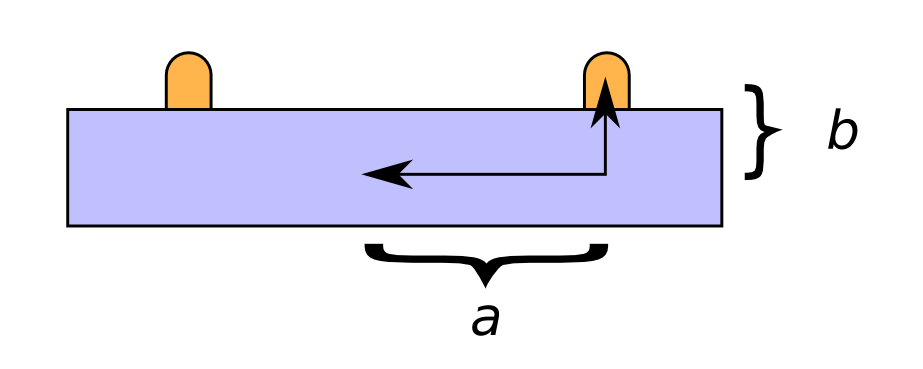
\includegraphics[width=4 cm]{annotate.png}
\end{minipage}
\end{tabular}

$\displaystyle \Delta x = \frac{P_{1x} + P_{2x}}{2} - \sin\phi_z \sin\phi_x b$

\hfill $\displaystyle \Delta y = \frac{P_{1y} + P_{2y}}{2} + \cos\phi_z \sin\phi_x b$

$\displaystyle \Delta z = \frac{P_{1z} + P_{2z}}{2} - \cos\phi_x b$

\hfill $\displaystyle \cos^2\phi_z = \frac{\left(\frac{P_{1y} - P_{2y}}{2a}\right)^2}{\left(\frac{P_{1x} - P_{2x}}{2a}\right)^2 + \left(\frac{P_{1y} - P_{2y}}{2a}\right)^2}$

\vfill
$\displaystyle \cos^2\phi_x = \frac{\left(\frac{P_{1x} - P_{2x}}{2a}\right)^2 + \left(\frac{P_{1y} - P_{2y}}{2a}\right)^2}{\left(\frac{P_{1x} - P_{2x}}{2a}\right)^2 + \left(\frac{P_{1y} - P_{2y}}{2a}\right)^2 + \left(\frac{P_{1z} - P_{2z}}{2a}\right)^2}$
\end{frame}

\begin{frame}
\frametitle{Built-in sanity check}
\only<1>{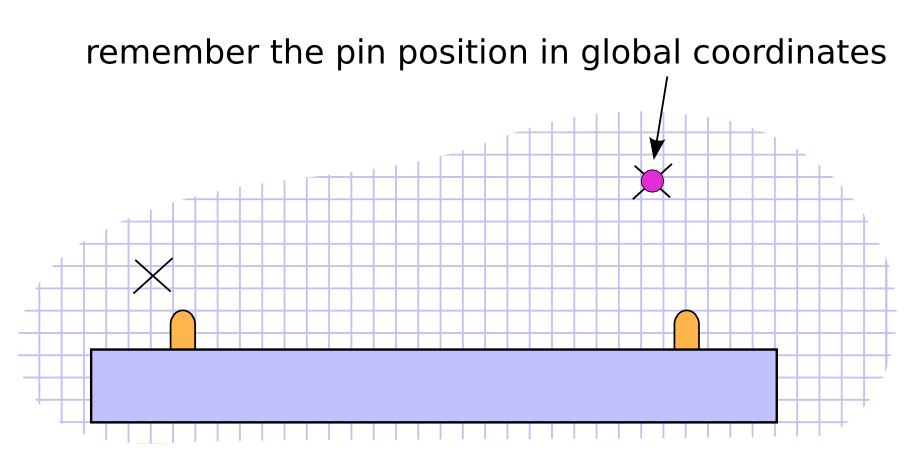
\includegraphics[width=\linewidth]{test3.png}}
\only<2>{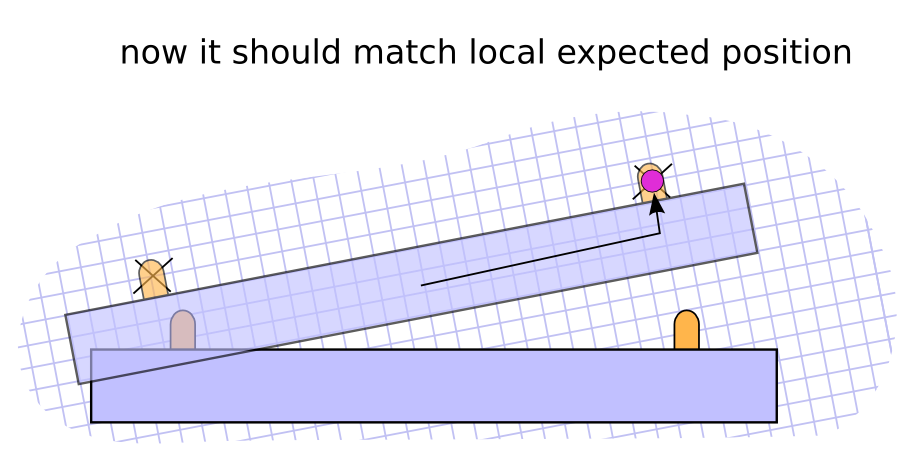
\includegraphics[width=\linewidth]{test4.png}}

\vfill
\begin{center}\uncover<2>{(This is a tautology.)}\end{center}
\end{frame}

\begin{frame}
\frametitle{Two ways of measuring error}

\begin{center}
\begin{tabular}{p{0.45\linewidth} p{0.45\linewidth}}
\begin{minipage}{\linewidth}
\begin{center}
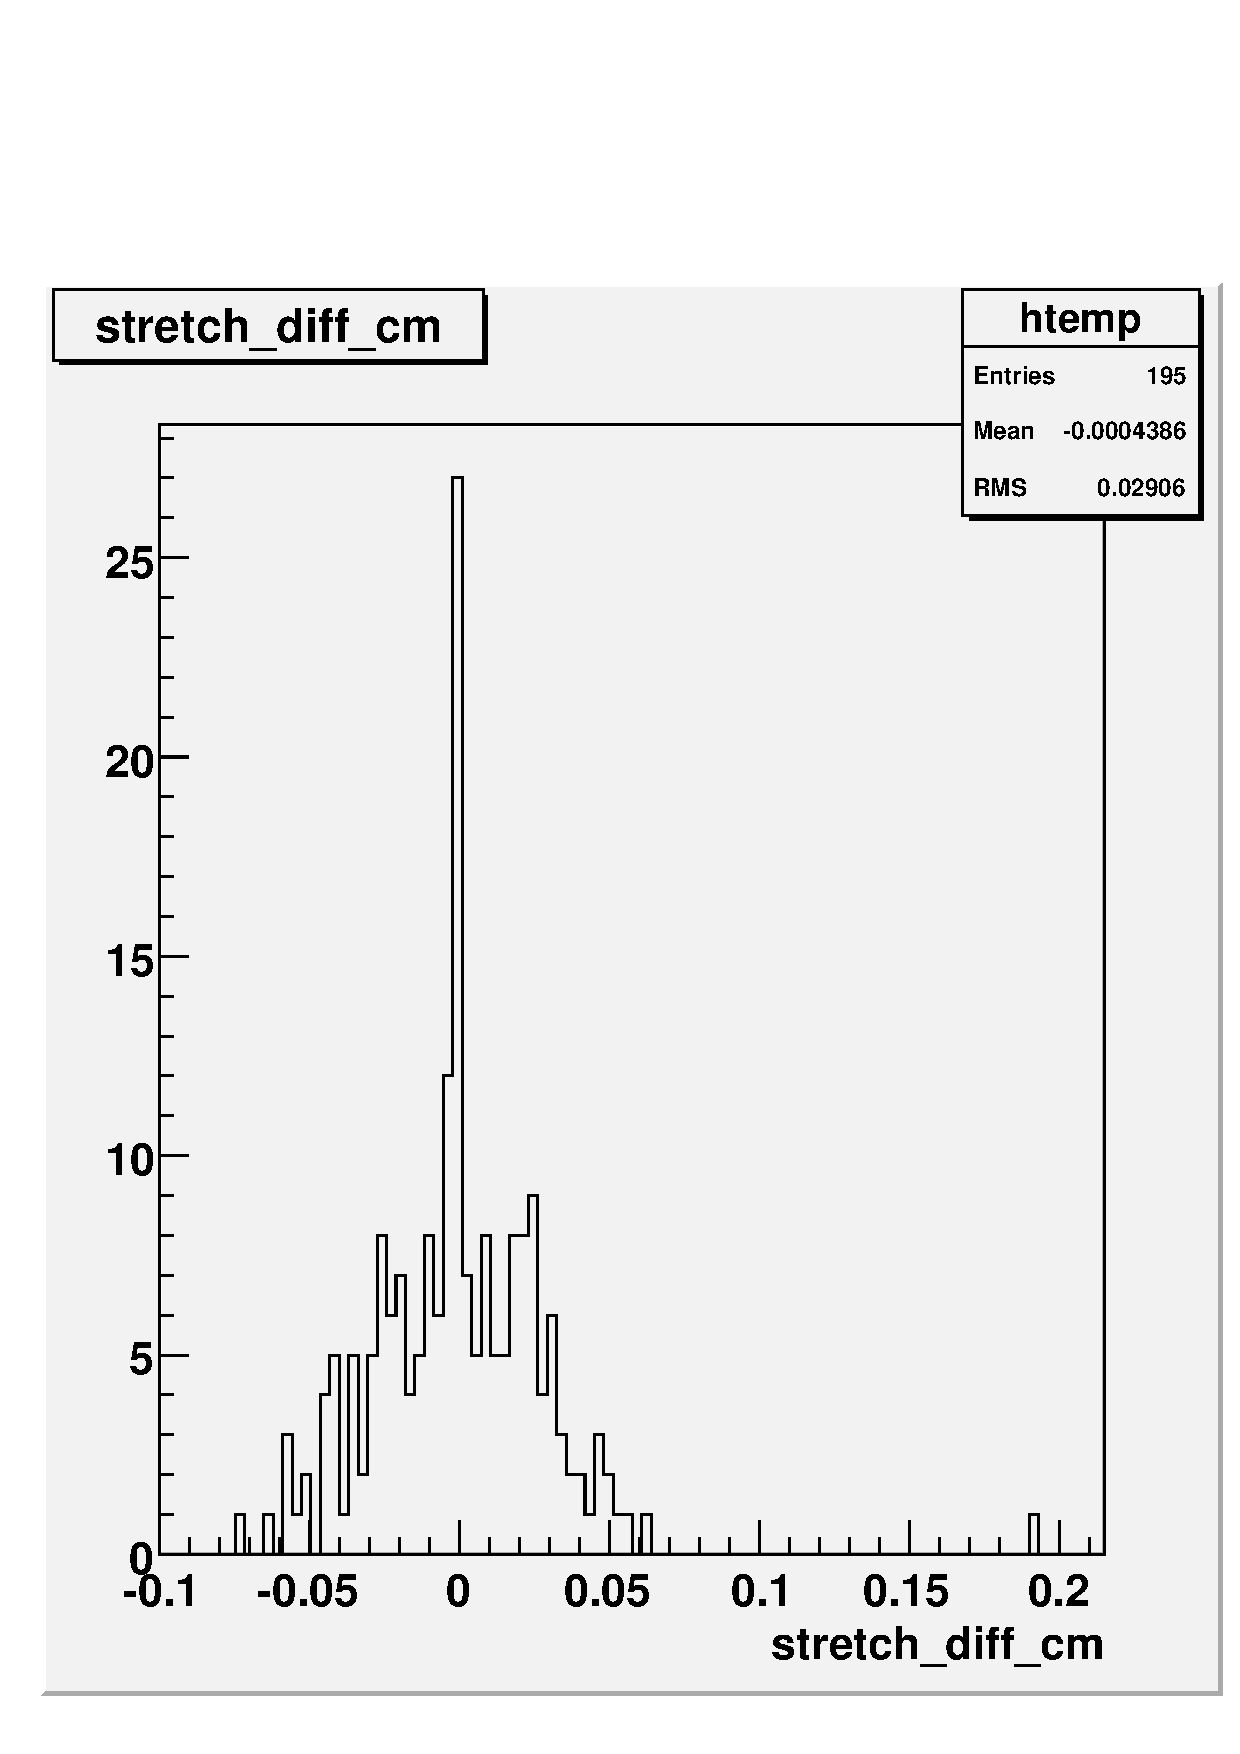
\includegraphics[width=0.9\linewidth]{stretch_factor.pdf}
\end{center}
\end{minipage} &
\begin{minipage}{\linewidth}
\begin{center}
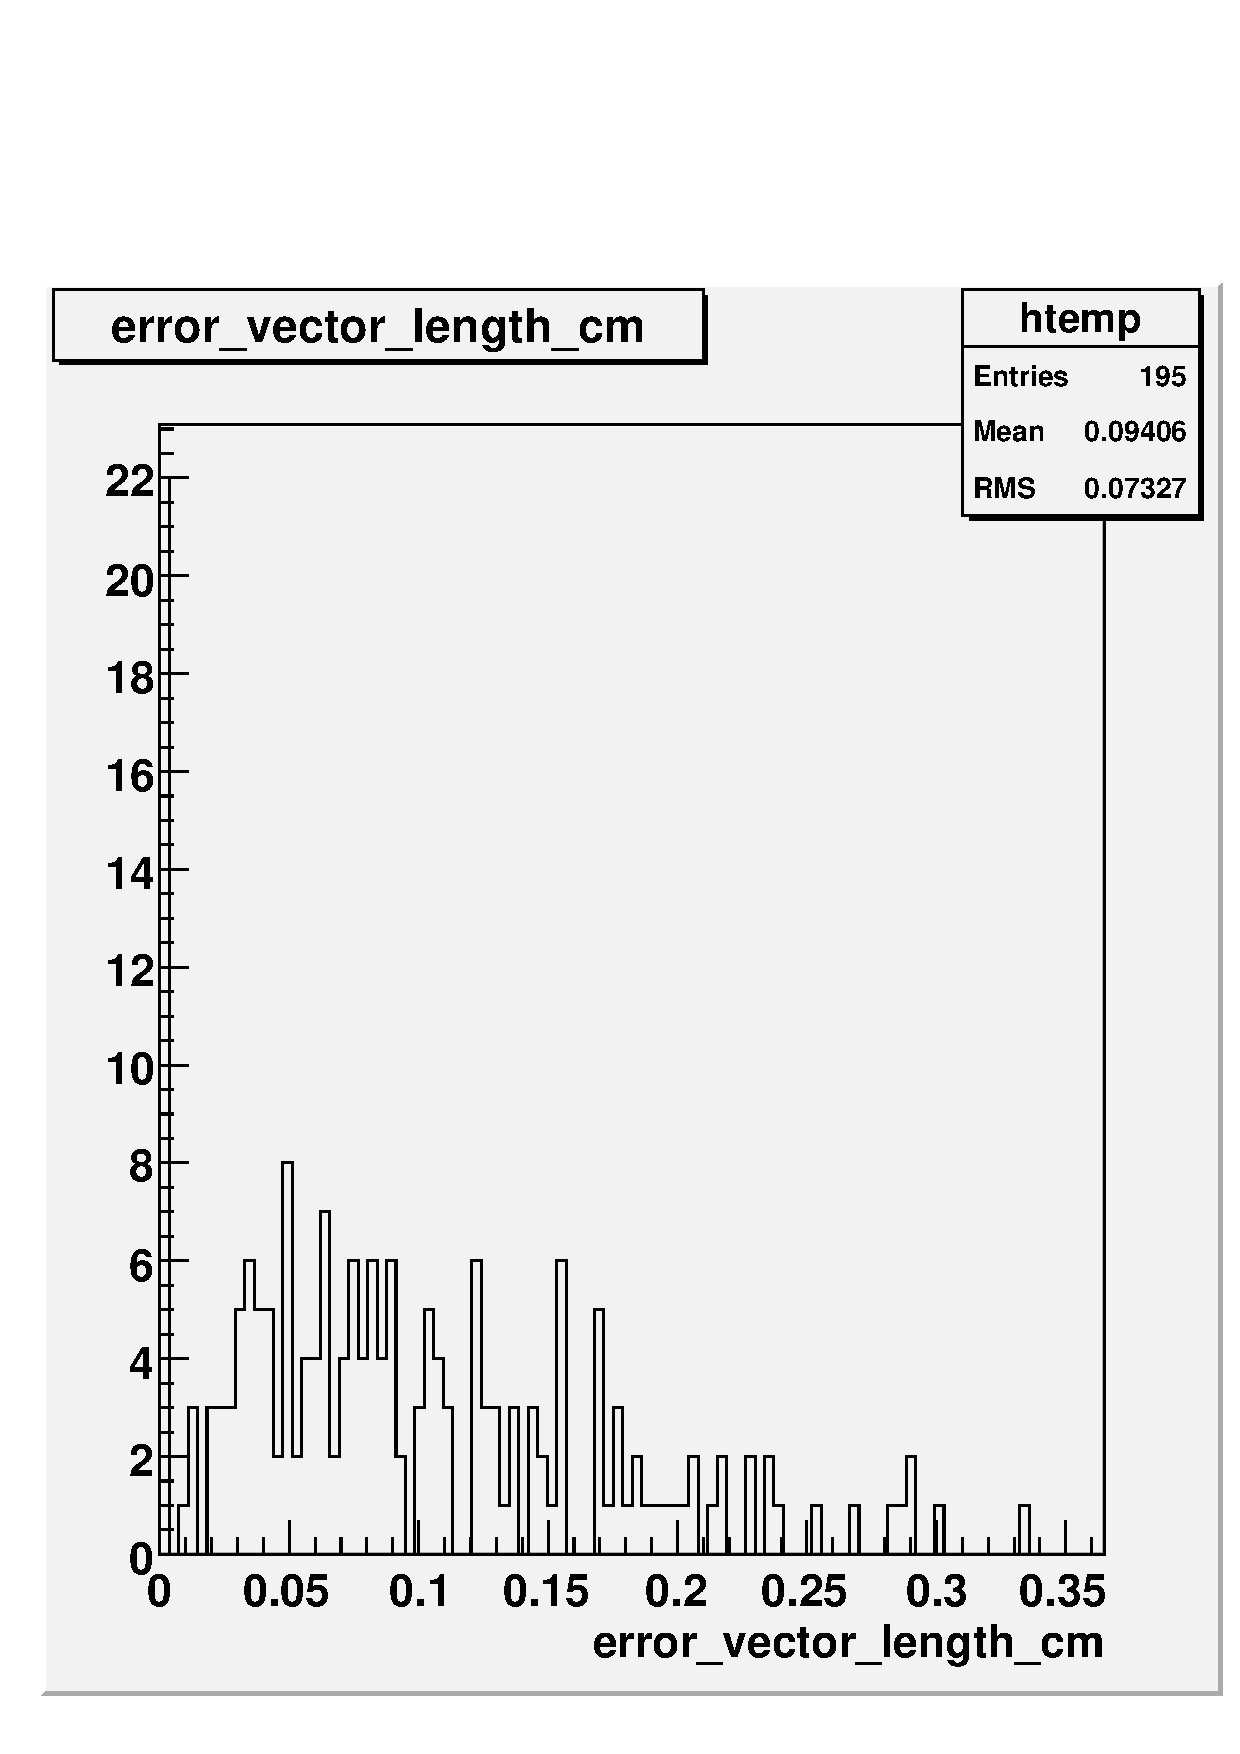
\includegraphics[width=0.9\linewidth]{error_length.pdf}
\end{center}
\end{minipage} \\
 & \\
\begin{minipage}{\linewidth}
\begin{center}
$(\mbox{stretch factor} - 1) \times \mbox{length}$
\end{center}
\end{minipage} &
\begin{minipage}{\linewidth}
\begin{center}
$\left|\mbox{mismatch of global point}\right|$
\end{center}
\end{minipage} \\
\begin{minipage}{\linewidth}
\begin{center}
$\to$ error in survey constraints
\end{center}
\end{minipage} &
\begin{minipage}{\linewidth}
\begin{center}
$\to$ error in our computation
\end{center}
\end{minipage} \\
\end{tabular}
\end{center}
\end{frame}

\begin{frame}
\label{numpages}
\end{frame}

\end{document}
